\documentclass{article}
\usepackage{amsmath,amsthm,amsfonts}

% graphical model drawing tools
\usepackage{tikz}
\usetikzlibrary{bayesnet}


\begin{document}
\begin{center}

\section*{Graphical Models}
\vspace{15mm}

Regular Markov Model\\

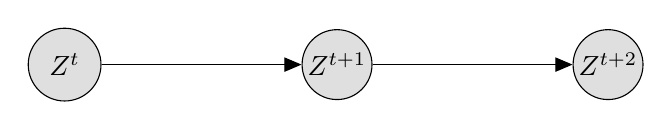
\begin{tikzpicture}[x=1in,y=1in]

% Nodes
  \node[obs]                     (Zt) {\hspace{.2cm}$Z^{t\hspace{.2cm}}$};
  \node[obs, right=of Zt]        (Ztplus1) {$Z^{t+1}$};                   
  \node[obs, right=of Ztplus1]   (Ztplus2) {$Z^{t+2}$};
      
% Edges
      \edge{Zt}       {Ztplus1};
      \edge{Ztplus1}  {Ztplus2};      

\end{tikzpicture}

%%%%
\vspace{20mm}

Hidden Markov Model\\

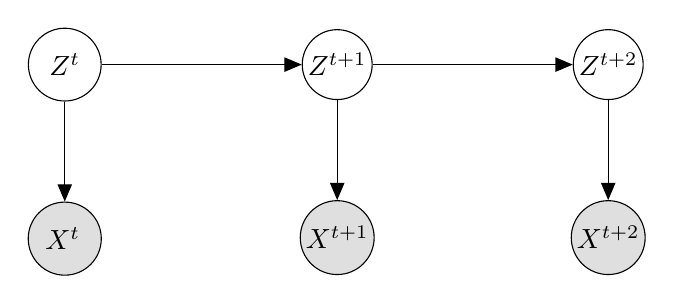
\begin{tikzpicture}[x=1in,y=0.5in]

% Nodes
  \node[latent]                    (Zt) {\hspace{.2cm}$Z^{t\hspace{.2cm}}$};
  \node[latent, right=of Zt]       (Ztplus1) {$Z^{t+1}$};
  \node[latent, right=of Ztplus1]  (Ztplus2) {$Z^{t+2}$};
  \node[obs, below =of Zt]         (Xt) {\hspace{.15cm}$X^{t\hspace{.2cm}}$};
  \node[obs, below =of Ztplus1]    (Xtplus1) {$X^{t+1}$};
  \node[obs, below =of Ztplus2]    (Xtplus2) {$X^{t+2}$};

% Edges
  \edge{Zt}       {Ztplus1};
  \edge{Zt}       {Xt}; 
  \edge{Ztplus1}  {Ztplus2};
  \edge{Ztplus1}  {Xtplus1};
  \edge{Ztplus2}  {Xtplus2};
      
\end{tikzpicture}

%%%%
\vspace{20mm}

Layered Hierarchical Models with Plates\\
\vspace{3mm}

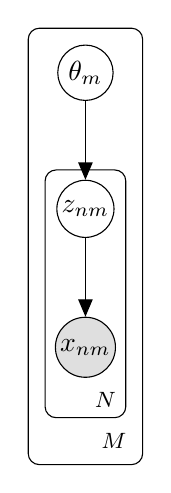
\begin{tikzpicture}

% Nodes
  \node[obs]                   (x)   {$x_{nm}$}; %
  \node[latent, above = of x]  (z)   {$z_{nm}$}; %
  \node[latent, above = of z]  (theta)   {$\theta_m$}; %

% Edges
  \edge{z}     {x} ;
  \edge{theta} {z} ;
  
% Plates
  \plate {xz} { %
    (x) %
    (z) %
  } {$N$} ;
  
  \plate [inner sep=0.2cm]{} {%
    (theta) %
    (z) %
    (x) %
    (xz.south east) (xz.south west) %
  } {$M$} ;

\end{tikzpicture}

%%%%
\vspace{5mm}

\begin{tikzpicture}

% Nodes
  \node[obs]                   (x)   {$x_{nm}$}; %
  \node[latent, above = of x]  (z)   {$z_{m}$}; %
  \node[latent, above = of z]  (sigma)   {$\sigma$}; %

% Edges
  \edge{z}     {x} ;
  \edge{sigma} {z} ;
  
% Plates

  \plate {x} { %
    (x) %
   } {$N$} ;
 
  \plate [inner sep=0.2cm]{xz} {%
    (z) %
    (x) %
    (xz.south east) (xz.south west) %
    } {$M$} ;

\end{tikzpicture}

%%%%

Basic Neural Network Structure\\
\vspace{3mm}
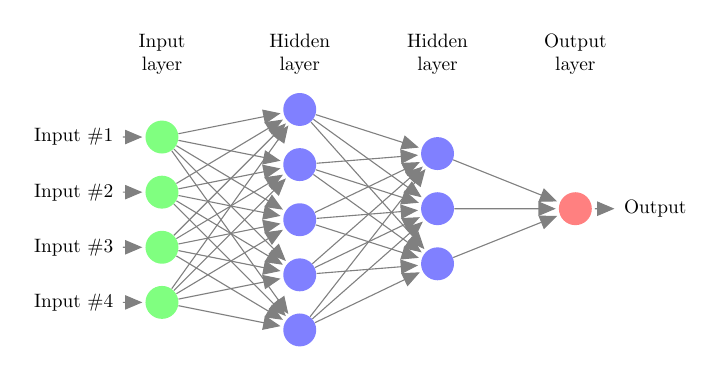
\begin{tikzpicture}[scale = .7,transform shape, shorten >=1pt,->,draw=black!50, node distance=2.5cm]
    \tikzstyle{every pin edge}=[<-,shorten <=1pt]
    \tikzstyle{neuron}=[circle,fill=black!25,minimum size=17pt,inner sep=0pt]
    \tikzstyle{input neuron}=[neuron, fill=green!50];
    \tikzstyle{output neuron}=[neuron, fill=red!50];
    \tikzstyle{hidden neuron}=[neuron, fill=blue!50];
    \tikzstyle{annot} = [text width=4em, text centered]

% Nodes
    % Input layer nodes
    \foreach \name / \y in {1,...,4}
        \node[input neuron, pin=left:Input \#\y] (I-\name) at (0,-\y) {};

    % Hidden layer nodes
    \foreach \name / \y in {1,...,5}
        \path[yshift=0.5cm]
            node[hidden neuron] (H1-\name) at (2.5cm,-\y cm) {};
     
    % Hidden layer nodes
    \foreach \name / \y in {1,...,3}
        \path[yshift=-.3cm]
            node[hidden neuron] (H2-\name) at (5cm,-\y cm) {};

    % Output layer node
    \node[output neuron,pin={[pin edge={->}]right:Output}, right of=H2-2] (O) {};

% Paths

    % Input layer with hidden layer
    \foreach \source in {1,...,4}
        \foreach \dest in {1,...,5}
           \path (I-\source) edge (H1-\dest);

    \foreach \source in {1,...,5}
        \foreach \dest in {1,...,3}
           \path (H1-\source) edge (H2-\dest);

    % Hidden layer with the output layer
    \foreach \source in {1,...,3}
        \path (H2-\source) edge (O);

% Layer labels
    \node[annot,above of=H1-1, node distance=1cm] (hl) {Hidden layer};
    \node[annot,left of=hl] {Input layer};
    \node[annot,right of=hl] (hl2) {Hidden layer};
        \node[annot,right of=hl2] {Output layer};

\end{tikzpicture}

\end{center}
\end{document}
